\begin{center}
    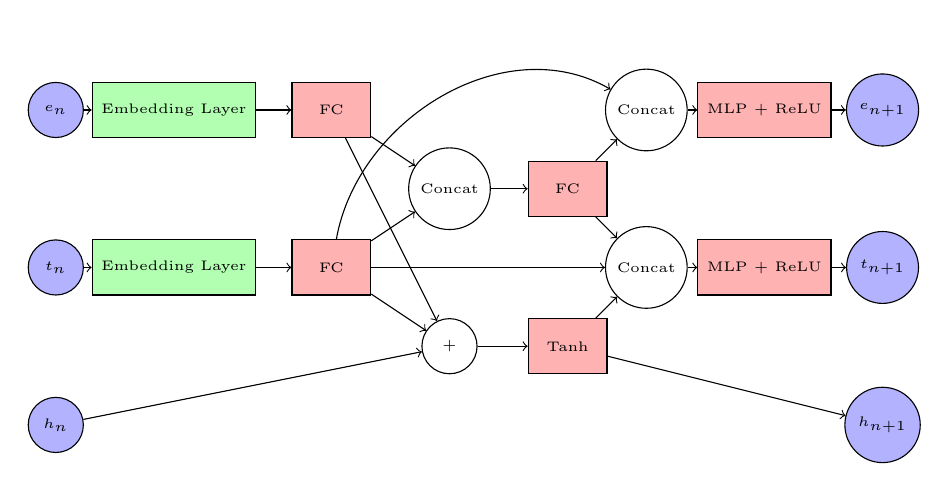
\begin{tikzpicture}[
            neuron/.style={circle, draw, minimum size=0.7cm},
            rect neuron/.style={rectangle, draw, minimum width=1cm, minimum height=0.7cm}, % Rectangular neuron
            input neuron/.style={neuron, fill=blue!30},
            embeddings neuron/.style={rect neuron, fill=green!30},
            mlp neuron/.style={rect neuron, fill=red!30},
            output neuron/.style={neuron, fill=red!30},
            every node/.style={align=center,font=\tiny}
    ]
        % Input Layer
        \node[input neuron] (inp_e) at (0.5,2) {$e_n$};
        \node[input neuron] (inp_t) at (0.5,0) {$t_n$};
        \node[input neuron] (inp_h) at (0.5,-2) {$h_n$};
        
        % Text Processing
        \node[embeddings neuron] (emb_e) at (2,2) {Embedding Layer};
        \node[embeddings neuron] (emb_t) at (2,0) {Embedding Layer};
        
        % Emotion Processing
        \node[mlp neuron] (MLP1_emo) at (4,2) {FC};
        \node[mlp neuron] (MLP1_txt) at (4,0) {FC};

        % Hidden Update
        \node[input neuron, minimum size=0.7cm,fill=white!30] (hidden_upd1) at (5.5,-1) {+};
        \node[mlp neuron] (hidden_upd2) at (7,-1) {Tanh};
        
        % Fusion
        \node[input neuron,fill=white!30] (concat1) at (5.5,1) {Concat};
        \node[mlp neuron] (mlp_fus) at (7,1) {FC};

        % Final Emotion
        \node[input neuron,fill=white!30] (concat2) at (8,2) {Concat};
        \node[mlp neuron] (MLP2_emo) at (9.5,2) {MLP + ReLU};

        % Final Text
        \node[input neuron,fill=white!30] (concat3) at (8,0) {Concat};
        \node[mlp neuron] (MLP2_txt) at (9.5,0) {MLP + ReLU};

        \node[input neuron] (out_emo) at (11,2) {$e_{n+1}$};
        \node[input neuron] (out_txt) at (11,0) {$t_{n+1}$};
        \node[input neuron] (out_hidden) at (11,-2) {$h_{n+1}$};

        % Arrows
        \draw[->] (inp_t) -- (emb_t);
        \draw[->] (emb_t) -- (MLP1_txt);
        \draw[->] (MLP1_txt) -- (hidden_upd1);
        \draw[->] (MLP1_txt) -- (concat1);
        \draw[->] (MLP1_txt) to[out=80, in=150] (concat2);
        \draw[->] (MLP1_txt) -- (concat3);
        

        \draw[->] (inp_e) -- (emb_e);
        \draw[->] (emb_e) -- (MLP1_emo);
        \draw[->] (MLP1_emo) -- (hidden_upd1);
        \draw[->] (MLP1_emo) -- (concat1);

        \draw[->] (inp_h) -- (hidden_upd1);
        \draw[->] (hidden_upd1) -- (hidden_upd2);
        \draw[->] (hidden_upd2) -- (concat3);
        \draw[->] (hidden_upd2) -- (out_hidden);
        
        \draw[->] (concat1) -- (mlp_fus);
        \draw[->] (mlp_fus) -- (concat2);
        \draw[->] (mlp_fus) -- (concat3);
        
        \draw[->] (concat2) -- (MLP2_emo);
        \draw[->] (MLP2_emo) -- (out_emo);
        
        \draw[->] (concat3) -- (MLP2_txt);
        \draw[->] (MLP2_txt) -- (out_txt);
        

    \end{tikzpicture}
\end{center}

